% !TEX TS-program = pdflatex
% !TEX encoding = UTF-8 Unicode
\documentclass[12pt]{report}
\usepackage[utf8]{inputenc} % set input encoding (not needed with XeLaTeX)

\usepackage{geometry} % to change the page dimensions
\geometry{a4paper} % or letterpaper (US) or a5paper or....
\geometry{margin=2cm} % for example, change the margins to 2 inches all round

% Packages
\usepackage{pdflscape}
\usepackage{graphicx} % support the \includegraphics command and options
\usepackage[parfill]{parskip} % Activate to begin paragraphs with an empty line rather than an indent
\usepackage{booktabs} % for much better looking tables
%\usepackage{array} % for better arrays (eg matrices) in maths
%\usepackage{paralist} % very flexible & customisable lists (eg. enumerate/itemize, etc.)
%\usepackage{verbatim} % adds environment for commenting out blocks of text & for better verbatim
\usepackage{subfig} % make it possible to include more than one captioned figure/table in a single float
\usepackage{amssymb}
\usepackage{epstopdf}
\usepackage{hyperref}
\usepackage{float}
\usepackage{caption}
\usepackage[table]{xcolor}
\captionsetup[table]{skip=10pt}
\usepackage{url}
\usepackage{wrapfig}
\usepackage{amsmath}

% Headers and Footers
\usepackage{fancyhdr} % This should be set AFTER setting up the page geometry
\pagestyle{fancy} % options: empty , plain , fancy
\renewcommand{\headrulewidth}{0pt} % customise the layout of headers and footers
\lhead{Final Report}\chead{}\rhead{Iain Johnston}
\lfoot{}\cfoot{\thepage}\rfoot{}

% Section Title Appearance
\usepackage{titlesec}
\titleformat{\section}{\large\bfseries}{\thesection}{1em}{\hrule}

% ToC appearance
\usepackage[nottoc,notlof,notlot]{tocbibind} % Put the bibliography in the ToC
\usepackage[titles,subfigure]{tocloft} % Alter the style of the Table of Contents
\renewcommand{\cftsecfont}{\rmfamily\mdseries\upshape}
\renewcommand{\cftsecpagefont}{\rmfamily\mdseries\upshape} % No bold!


% The document content starts below

\title{\textit{Final Report}\\\textbf{Maximising entertainment value in the vote-reveal problem}\\ Final Year Project (CM3203) - 40 Credits}
\author{Author: Iain Johnston (1312579) \\ Supervisor: Richard Booth\\ Moderator: Xianfang Sun}
\date{} % Activate to display a given date or no date (if empty),  otherwise the current date is printed

\begin{document}
\maketitle
\clearpage

\section*{Abstract}

\section*{Acknowledgements}

\tableofcontents %  place a table of contents after the title
\listoffigures
\listoftables
\clearpage % clear the page after the table of contents

%\addcontentsline{toc}{section}{Section z} % how to add an entry to the table of contents that is un-numbered
%\section*{Second Section} % an un-numbered section in the document
%\subsection{A subsection} % an example subsection
\section{Introduction}\label{Introduction}
% tell the reader what the project is about without assuming special knowledge and without introducing any specific material that might obscure the overview.
% anticipate and combine main points described in more detail in the rest
% include things such as:
% the aim(s) or goal(s) of the project,
% the intended audience or “beneficiaries” of the work done,
% the scope of the project,
% the approach used in carrying out the project,
% assumptions on which the work is based and
% a broad summary of important outcomes.
In many elections or competitions, a set of voters will rank a set of candidates from best to worst, or will give scores to some of the candidates, with the winner then being the candidate that gets the highest total number of points. When it comes to revealing the result after all votes have been cast, some competitions proceed by having a roll-call of all the voters in which each announces their own scores. This is often done for entertainment purposes such as in the Eurovision Song Contest.\cite{EurovisionVoting}

The concept of \textit{entertainment}, especially with respect to competition, is a heavily subjective matter and as such is difficult to quantify in simple terms. There are intuitive constituent parts to an \textit{entertaining} competition (like Eurovision) such as, if the winner is known early or late, and how many teams are in the running to win. This project will find ways to translate these slightly nebulous concepts into more concrete mathematical functions.  

The two main questions that this project will aim to answer are:

\begin{enumerate}
\item How can we define the concept of ''entertainment'' in the context of an optimisation problem, and hence try to maximise it.
\item  In which order should the votes be revealed in order to maximise that entertainment value?
\end{enumerate}

To try and answer these questions the Eurovision Song Contest will be used as an example as it has good quality datasets. Furthermore voting rules have gone through changes over the years as more countries joined and as it grew in popularity, giving the project a natural comparison tools throughout. Most recently since the 2016 running of the contest. The scoring rules of Eurovision are also well documented and relatively simple (see \ref{Background} for deeper explanation).

These changes to the voting rules show that the motivation behind this project, to maximise entertainment when revealing the votes, is a current problem and there have been attempts to try and solve this problem already.

There is no specific intended audience of this project, Eurovision is a test competition as it fits well with the more general optimisation problem that this project is trying to solve. In this regard it could be said that the beneficiaries of the project would be those who would also attempt to solve this problem, for other datasets or competitions. This project can help set out a framework for approaching these problems and many parts could even be re-used as long as the problem can be formulated in a specific way (see \ref{Implementation} for details on how)

The scope of this project is to try and solve the problem by finding a globally optimum solution, or by find the best solution possible and hence have a voting order that is the most entertaining. Also within scope is producing a way of visualising the solutions found and from this gaining better insight into why they are entertaining. This project does not try and influence other parts of the voting that could also lead to more entertainment (such as who delivers the votes or other human traits, only the order itself)

The approach to tackle this problem is a scientifically minded one. There are three main sections to the project. Firstly, designing and implementing functions that quantify the entertainment of a given voting order. Secondly, solving the optimisation problem of maximising the entertainment value given by those functions; using optimisation algorithms. Finally, analysing the solutions given and comparing and contrasting why there are entertaining and how well the algorithms did in finding them. This approach involves iteration on theoretical ideas whilst feeding back in results as the project goes along.

The important outcomes of this project are, a solution that delivers an entertaining competition when the votes are revealed, a way of describing entertainment mathematically, and a way of visualising the competition as the votes are revealed.

\section{Background}\label{Background}
% give reader info that they can't be expected to know, but which they need in order to fully understand and appreciate the report
% explain why the project is addressing the problem described in the report
% indicate an awareness of other relevant work
% show clearly that the problem has not been solved by anyone else
% include things such as:
% the wider context of the project,
% the problem that has been identified,
% likely stakeholders within the problem area,
% any theory associated with the problem area,
% any constraints on the approach to be adopted,
% existing solutions relevant to the problem area, and why these are unsuitable or insufficient in this particular case,
% methods and tools that your solution may be based on or use to solve the problem,
% you should also refer to the general problem for which these algorithms are useful (the application(s) for your techniques).
% existing products, documents or artefacts that you should mention could be:
% similar to the one you are proposing,
% support your project,
% your project aims to extend or replace,
% demonstrate the “deficiencies” your project intends to address.
The more general reason for this project is to try and see if there can easily be found an optimal solution to a problem when given a mathematical representation of something that humans experience. 

Moreover in competitions where voting is revealed, such as in Eurovision, one of the only ways to change how entertaining the competition seems, is to change the order. Any other changes to the actual running of the competition are unethical.

Furthermore as competitions are usually televised or watched live, it is generally in the interest of those in charge of the competition to produce an entertaining show as this helps them with many facets of their business such as through advertising, but also in building a following for the competition. In this way, it is obvious that a more exciting competition leads to more engaged fans.

\subsection{Project Context}\label{Project Context}
Eurovision has been a topic of research for many years now. The main focus of that research has been in relation to the voting patterns that can be found over the course of many runnings of the competition. This research such as \textit{"Comparison of Eurovision Song Contest Simulation with Actual Results Reveals Shifting Patterns of Collusive Voting Alliances"}\cite{gatherer2006}, \textit{"Geography, culture, and religion: Explaining the bias in Eurovision song contest voting"}\cite{so66198} and \textit{"The Eurovision Song Contest. Is voting political or cultural?"} \cite{Ginsburgh200841} all use the Eurovision Song Contest as a basis to investigate political and cultural phenomena.

There have also been some more computational view of Eurovision such as \textit{"Using the Clustering Coefficient to Guide a Genetic-Based Communities Finding Algorithm"}\cite{Bello2011} which attempts to find communities within the voting patterns.

The particular problem this project is addressing has not been approached in a scientific setting as yet. It does seem to have been at least tackled by those that run Eurovision however not with exactly the same data and considerations. Moreover as they are a private company they have never published any methodology on how they pick voting orders. They usually state on their website when revealing the voting order that 
\begin{verbatim}"The voting order has been determined by the results from last night's Jury Final.
An algorithm has been created to try and make the voting as exciting as possible."
\end{verbatim}\cite{votingOrderQuote}
There is no mention of how this algorithm works or what they constitute entertaining or exciting.

The biggest drawback that can be said about the current Eurovision algorithm, without seeing it and understanding its methodology, is that it only takes into account Jury votes as they can be decided on during the dress rehearsals. This is problematic as the Jury and tele-voting can diverge for many reasons and hence the voting order that purports to be entertaining, may only be such when the viewers at home agree exactly with the Jury.

This project's method takes into account both the sets of votes and hence could give a more correct picture of what will happen, entertainment wise, for any given voting order. One main deficiency with this method is that fact, as it is necessary to wait for all the votes to be cast and then the voting order can be found. In real world terms this may not be feasible for the Eurovision Song Contest as they may have commitments that require that the voting order is known in advance for various logistical reasons.

Another drawback as mentioned above, is the fact that there is no explanation as to why their algorithm believes a given order to be more exciting than any other. This project will attempt to standardise mathematically a function for entertainment, which could in future be compared through human tests (see \ref{FutureWork}).By describing a concept mathematically not only can it be used by algorithms but it can also form part of a proof of which a general thought put forward by a human cannot be.

This project only looks at one specific area of the competition to describe and codify entertainment. This can be seen as a drawback of the solutions found, however the way this project has been undertaken leaves the opportunity of further work in the area of defining entertainment functions as described in \ref{FutureWork}.

The techniques used and implemented in this project have applications outside the strict problem that is being solved here. For example even though this problem is specifically trying to produce entertaining orders for Eurovision, there is no reason why other competitions who use the same type of ordered voting system (sometimes referred to as roll-call voting) could use the algorithms and framework designed and implemented in this project to solve their problems. 

\subsection{Background Theory}\label{BackgroundTheory}
Understanding how the Eurovision Song Contest voting works is key to this project, as this affects many parts of the design and implementation of entertainment functions. Furthermore the system for voting has been changed over many years and so to try and standardise the project I will be using the system that was in use during the 2014 running of the competition, and the main dataset also comes from that year.\footnote{2014 voting system is the system that had been in use from 2009 and changed in 2016}

In this system, each country awards two sets of 12, 10, 8–1 points to their 10 favourite songs: one from their professional jury and the other from tele-voting. Moreover as voting is done by both and jury and by people voting by phone, both constituent parts count 50\% towards the final score.

In the 2014 contest, there were 37 countries that participated and of those 26 reached the final. All 37 countries vote in the final. From this point on in this report, the countries that vote are referred to as \textit{voters} and those 26 competing in the final are referred to as \textit{participants}. There is overlap between the two groups i.e the \textit{participants} set is a subset of the \textit{voters} set; but it should be obvious from the context to whom is being referred.

\begin{figure}[H]
\centering
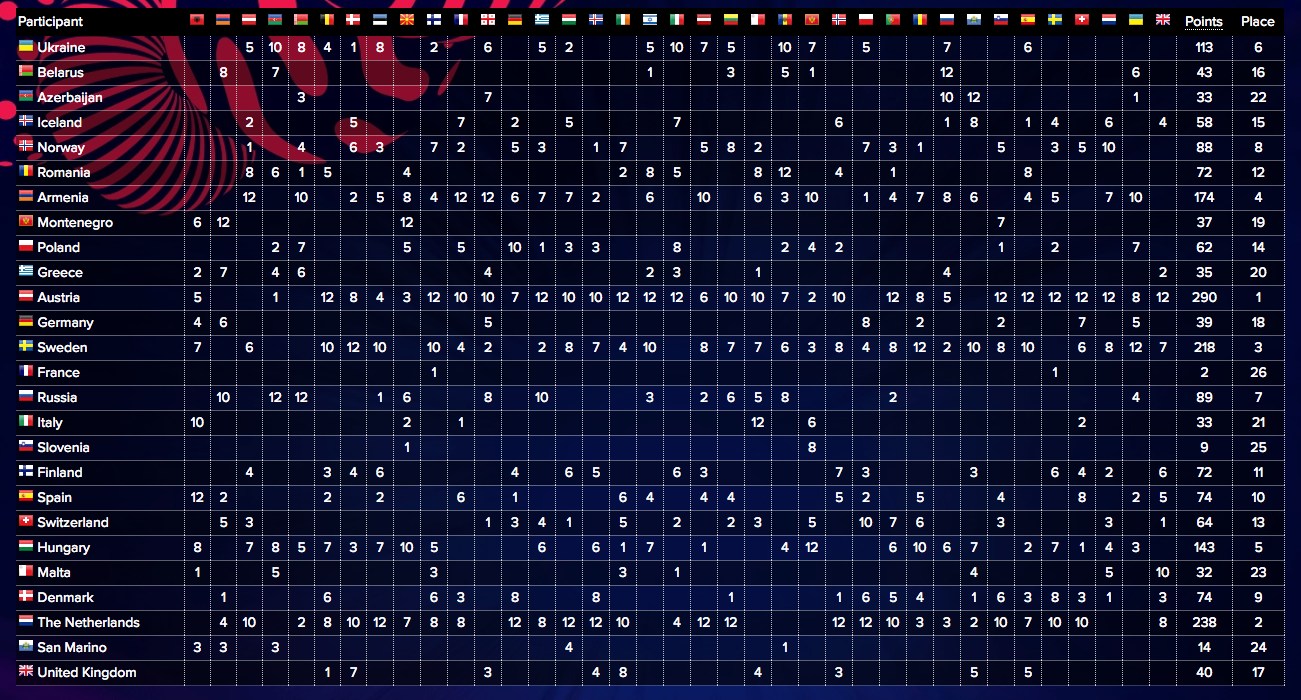
\includegraphics[width=15cm, height=7cm]{./2014Scoreboard}
\caption{2014 Scoreboard}
\label{f_2014Scores}
\end{figure}

This voting system creates a matrix of scores as seen in Figure \ref{f_2014Scores}. The \textit{voters} are arranged along the top alphabetically, while the \textit{participants} are along the left hand side. Points refers to the final total of all the scores given at the end of all voting, and rank is their final position in the competition. 

This is important to look at as it can help clarify what this project's aim is. A solution to the problem is found by moving the \textit{voters} along the top into different positions and then analysing the scores after each country has voted, to reach an \textit{entertaining} order for those countries to reveal their votes.

% Your background section should end with a clear statement of the research questions problem your project is trying to answer. 
%These will reflect the aim of your project, but will be different in that they explain the problem you are attempting to solve
Hence the problem that this project is trying to solve is about ordering who votes when so as to maximise some mathematical concept of entertainment. Should the order put Spain and France next to each other in the order, or would it be better if they were split up. Should Ukraine's vote be near the start or near the end so that the competition is exciting. This is what the project is trying to decide.

\section{Algorithm Designs/Approach}\label{AlgorithmDesigns}
% give reader a clear picture of the system
% specification becomes: description of the problem and what is required of a solution
% design becomes: description of your approach to solving the problem and your suggested solution(s)
% problem statement section and then a section describing one or more suggested algorithms to solve the problem
% Later in results and evaluations describe how to design experiments to test how well the algorithms solve the problem and present experimental results with an evaluation of your suggested solutions
% big-O
% reasoning behind writing each algorithm
To clarify the problem it is easier to view a much smaller competition and then run through the main points of theory, that then are used in the full Eurovision system.

Firstly we design a competition that involves 3 teams total, of which 2 are \textit{participants}. The scoring system is even more simple than the one used by Eurovision. Here each voting team gives 1 point the team they prefer and 0 to the other. A team cannot give itself 1 point. This produces a matrix of scores similar to the one in Figure \ref{f_2014Scores}. It is shown in Table \ref{t_simpleMatrix}.

\begin{table}[H]
\centering
\caption{Scores for simple example game}
\label{t_simpleMatrix}
\begin{tabular}{@{}|l|l|l|l|@{}}
\toprule
        & Austria & Spain & France \\ \midrule
Austria & 0       & 1     & 1      \\ \midrule
France  & 1       & 0     & 0      \\ \bottomrule
\end{tabular}
\end{table}

From Table \ref{t_simpleMatrix} we can see how the scores will be calculated in this type of competition. For simplicity, the order that the teams vote is the order from left to right in Table \ref{t_simpleMatrix}. This means that after Austria has voted the scores are $Austria: 0, France: 1$, the rest of the competition is shown in Table \ref{t_simpleScores}

\begin{table}[H]
\centering
\caption{Scores per round}
\label{t_simpleScores}
\begin{tabular}{@{}|l|l|l|l|@{}}
\toprule
        & After Austria's vote & After Spain & After France \\ \midrule
Austria & 0       & 1     & 2      \\ \midrule
France  & 1       & 1     & 1      \\ \bottomrule
\end{tabular}
\end{table}

We can see that France wins this competition, with 2 points. This cumulative scoring extends to the full Eurovision competition in the exact same way, except for in that case there are 30+ voters.

All that is needed to turn this simple example into Eurovision is to add all the \textit{voters} and \textit{participants} and change the scores given out to be $12, 10, 8-1$ instead of just 1 and 0.

\subsection{Entertainment Function}\label{EntertainmentFunction}
From the small example, it is quite easy to think of some theoretical reasons why a given order is entertaining. This leads straight into the design of entertainment functions and how they model entertainment. 

It is important to start with the design of the entertainment functions as they are the main workhorse part of finding solutions to the problem. The approach was to analyse the competition and try and identify things in a competition that lead to excitement. From those ideas, it was a case of trying to formalise that theory into a concrete piece of maths that could then be programmed. Furthermore the entertainment functions are quite problem specific and may not transfer well into other problems, whereas the algorithms are entirely agnostic to the problem at hand. This means the entertainment functions follow much more closely from the problem itself than any other part of the project.

Any entertainment functions talked about in this section share some characteristics that need to be explained. The first is that they take a \textbf{solution ($\Phi$)} to the problem (see Glossary-3) as input and they return a single \textbf{entertainment value} ($\varepsilon$) (see Glossary-4). Moreover they calculate the \textbf{scores}($S$) (see Glossary-6) for each \textit{participant} country every \textbf{round} ($R$)(see Glossary-5).

The first entertainment function that was designed is named \textbf{MaxMin} and as it's name suggests it works by finding the difference between the highest score (max) and the lowest score (min) after each voting round. It then sums the value which is the $\varepsilon$ value for that solution. This function follows quite naturally from watching and analysing the Eurovision competition as the way roll-call style voting works, everything is building towards the later end of the voting order. Hence it seems to be a innate part of the competition that you would want every country to be in with a chance of winning for as many rounds as possible. Moreover as there is only one prize, for first place, it is even less important to worry about positioning other than the top.

So each round the distance ($\Lambda$) is calculated as such:
\begin{equation}
	\Lambda = \max(S) - \min(S)
\end{equation}

Then keeping the distance per round $i$ as $\Lambda_i$, the entertainment value ($\varepsilon$) is found by:
\begin{equation}
	\varepsilon = \sum_{i=0}^{n_R}  \Lambda_i
\end{equation}

This is a relatively simple equation and hence transfers simply to code. However more importantly, it encodes an intuitive part of entertainment mathematically. These functions encode the fact that an entertaining competition is one in which the distance between first and last place is as low as possible as often as possible. In this case instead of maximising $\varepsilon$, we want to minimise it.

Over the course of a whole competition i.e: $n_R$ voting rounds, it is intuitive to want that distance to stay as low as possible. Hence finding the sum of the distance ($\Lambda$) in each round and then using optimisation algorithms to try and find a solution ($\Phi$) that minimises this value.

However there is one major drawback of the basic MaxMin method, which is that in some rounds, especially later in the competition, the last place country is actually mathematically eliminated from the race for first place.

This leads to a second version of the entertainment function for this problem. As it is essentially a refinement of the first function and not a brand new method it is called \textbf{RefinedMaxMin}.

Where \textbf{RefinedMaxMin} and \textbf{MaxMin} differ is how the $\min$ part of equation 1 is calculated. As some of cannot win the competition, they should not be taken into account when seeing if a solution is entertaining or not.

To find whether a team can still win, the upper bound of points left available is found. This means that we assume for each team, and for the remaining rounds left to be revealed, that they gain the maximum (12) points and the hence we find the highest score they could ever attain. This method does not take into account whether the country has already given itself a vote (in which case they would not be allowed to get 12 points in that round). This was done to simplify the method and make testing it's improvements against MaxMin easier.

The method for finding if a team can still win is to first sort the scores for every country in round $i$ in ascending order. Then iterating through that list of scores from the start and for each round checking whether equation 3 is true.
\begin{equation}
	countriesScore + (maxScorePerRound * roundsRemaining) < currentTopScore
\end{equation}

If equation 3 hold true then that country cannot win and it is the minimum score


\begin{figure}[H]
\centering
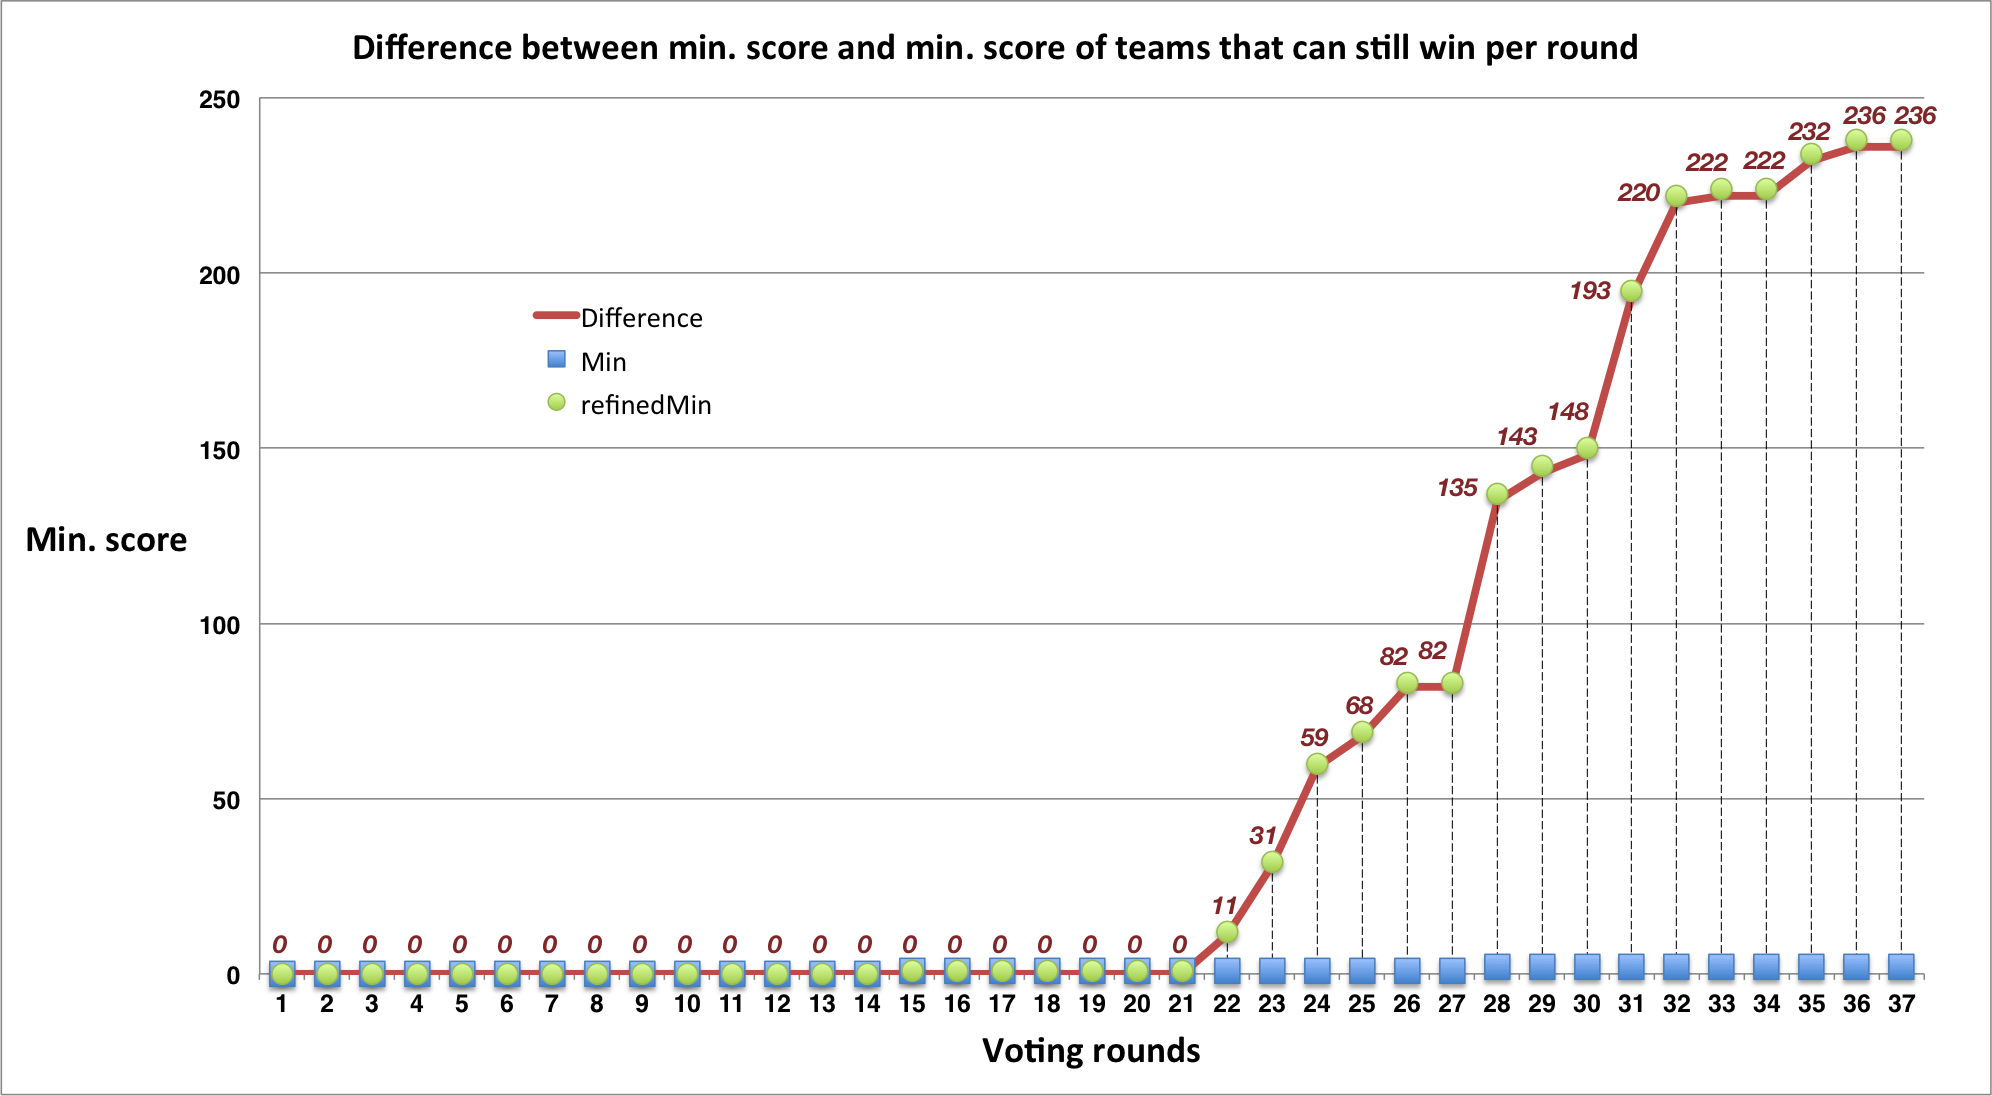
\includegraphics[width=17cm, height=9cm]{../code/misc/difference_MinvsRefinedMin}
\caption{Difference is $\Lambda$ found for MaxMin method and RefinedMaxMin}
\label{f_maxminDif}
\end{figure}

\subsection{Optimisation Algorithms}\label{Algorithms}


\section{Implementation of Algorithms}\label{Implementation}
% describes system but does so at finer level of detail, down to code level
% realisation of concepts and ideas developed earlier
% complete source code should be provided separately
% pick out and describe pieces of code which for example:
% are especially critical in operation of system
% are of particular interest
% illustrate a non-standard or innovative way of implementing an algorithm, data structure
% mention unforeseen problems that you encountered when implementing the system like:
% difficulties involving existing software
% lack of suitable supporting framework
% over ambitious project aims
% A seemingly disproportionate amount of project time can be taken up in dealing with such problems. The Implementation section gives you the opportunity to show where that time has gone.

\section{Results and Evaluation}\label{Results}
% describe to what extent you achieved your goals
% describe how you demonstrate that the system works as intended (or not)
% include comprehensible summaries of the results of all critical test that were carried out
% should try to indicate how confident you are about whatever you have produced, and also suggest what tests would be required to gain further confidence
% describe the reasoning behind the tests to evaluate your results, what tests to execute, what results show and why to execute these tests
% include discussion of how you are designing your experiments to verify hypothesis of more scientifically oriented project
% eg. describe how you compare the performance of your algorithm to other algorithms to indicate better performance and why this is a sound approach. then summarise the results of the tests of experiments
% critically evaluate your results in the light of these tests, describing its strengths and weaknesses. ideas for improvement can be carried over into Future work.
% present a critical appraisal of the project as a whole, including why the programming language and methodology chosen were appropriate

\section{Future Work}\label{FutureWork}
% expressing unrealistic ideas, including what you would have liked to have done if only you had not run out of time
% provide a good starting point for someone else to continue the work which you have begun

% is the solution optimal
% evaluating the entertainment function using real world people
% more entertainment functions

\section{Conclusions}\label{Conclusions}
% summary of the aims of the project and a restatement of the main results, i.e. what has been learnt and acheived
% an effective set of conclusions should not introduce new material. Instead it should briefly draw out, summarise, combind and reiterate the main points that have been made in the body of the project report and present opinions based on them

\section{Reflection on Learning}\label{Reflection}
% identify the impact of what we have done on the assumptions, concepts and ideas we used to make decisions about our work
% try to identify the characteristics of the problem that has been addressed , and consider whether assumptions of decisions about the relevant approach to solving the problem had been appropriate, in order to make a better decision in relation to problems that might be encountered in the future.

\section*{Glossary}
\addcontentsline{toc}{section}{Glossary}
\begin{enumerate}
\item \textbf{Voters ($V$)}: All countries that are in the Eurovision song contest who vote in the final. The voters is a list of countries. It looks like ["Ukraine", "Austria", "France",....]
\item \textbf{Participants ($P$)}: A subset of the voters that perform songs in the final and receive points from the other voters.
\item \textbf{Solution ($\Phi$)}: A solution to the optimisation problem this project is attempting to solve. A solution consists of two things:
	\begin{itemize}
		\item An ordering of the voting countries as a list
		\item An entertainment value found by an entertainment function
	\end{itemize}
\item \textbf{Entertainment Value ($\varepsilon$)}: A value given to a solution that describes how entertaining it is. Calculated using an entertainment function given a solution.
\item \textbf{Round ($R$)}: One round is when one \textit{voter} has given all the \textit{participants} a score. The competition is made up of $n_R$ rounds where $n_R = V$.
\item \textbf{Scores ($S$)}: How many points each country has received per round. The scores are an array of the same length as the number of \textit{participants}. It looks like [0,0,2,12,7,4,0,0,3,2,10,....]. When referring to it in the report along with \textbf{rounds} it is most likely cumulative so that after the final round the scores are the total scores for each country.
\end{enumerate}

\section*{Table of Abbreviations}
\addcontentsline{toc}{section}{Table of Abbreviations}

\section*{Appendices}
\addcontentsline{toc}{section}{Appendices}
%\begin{landscape} 
%\section*{Appendix}
%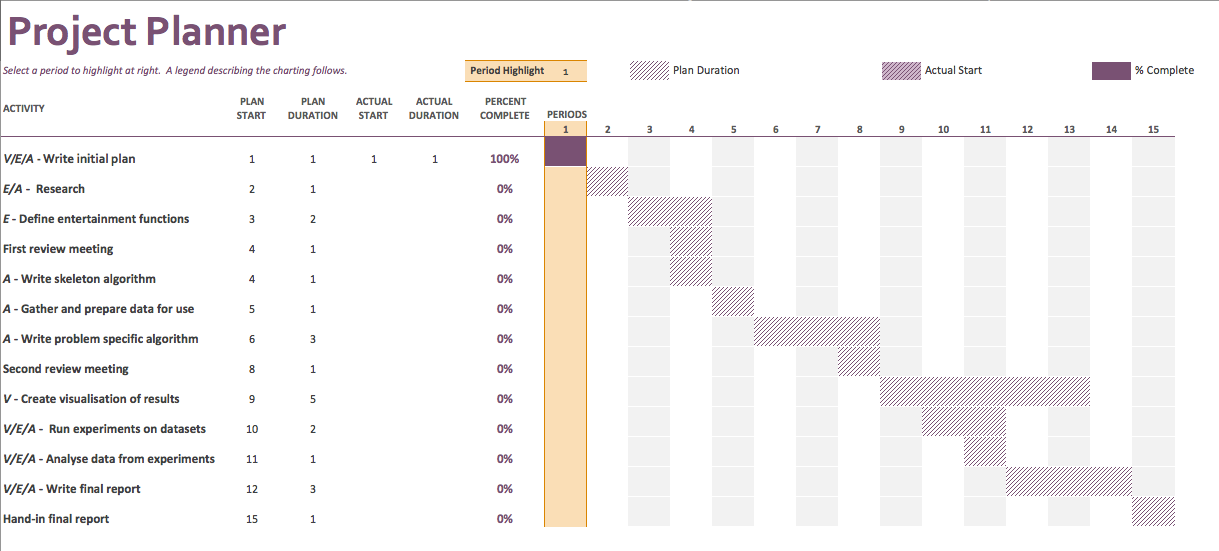
\includegraphics[height=14.5cm, width=\linewidth]{InitialPlanGanttChart.png}
%\end{landscape}

\clearpage
\renewcommand{\bibsection}{\section*{References}}
\addcontentsline{toc}{section}{References}
\bibliography{./References/finalReportBib}{}
\bibliographystyle{ieeetr}

\end{document}
